\documentclass[nooutcomes]{ximera}
%% handout
%% space
%% newpage
%% numbers
%% nooutcomes


\newcommand{\RR}{\mathbb R}
\renewcommand{\d}{\,d}
\newcommand{\dd}[2][]{\frac{d #1}{d #2}}
\renewcommand{\l}{\ell}
\newcommand{\ddx}{\frac{d}{dx}}
\newcommand{\dfn}{\textbf}
\newcommand{\eval}[1]{\bigg[ #1 \bigg]}

\usepackage{multicol}

\renewenvironment{freeResponse}{
\ifhandout\setbox0\vbox\bgroup\else
\begin{trivlist}\item[\hskip \labelsep\bfseries Solution:\hspace{2ex}]
\fi}
{\ifhandout\egroup\else
\end{trivlist}
\fi} %% we can turn off input when making a master document
\usepackage{fullpage}

\title{2.2:  Definition of Limits}  

\begin{document}
\begin{abstract}		\end{abstract}
\maketitle

%Problem 1
\begin{problem} \hfil
	\begin{enumerate}

	\item  True or False: To find $\lim_{x \to 2} f(x)$, it's enough to know the values of $f(2.1)$, $f(2.01)$, $f(2.001)$, and so on.
	\begin{freeResponse}
	 False.  These values will only help us make a guess at $\lim_{x \to 2^+} f(x)$, the right hand limit of $f$ as $x$ approaches $2$.  To determine $\lim_{x \to 2} f(x)$, we also need to know $\lim_{x \to 2^-} f(x)$ which we cannot determine from the above values.  For example, consider the function
	 	        \[
          f(x) =
        \begin{cases}
         -1 & \mbox{if $x < 2$,}\\
          0 & \mbox{if $x = 2$, and}\\
          1 & \mbox{if $2 < x$.}
        \end{cases}
        \]

	Looking at the graph of this function below, we can see that $\lim_{x \to 2^+} f(x) = 1$ and $\lim_{x \to 2^-} f(x) = -1$.  Thus, since $\lim_{x \to 2^+} f(x) \neq \lim_{x \to 2^-} f(x)$, $\lim_{x \to 2} f(x)$ does not exist.
	
		\begin{image}
          \includegraphics[scale = 0.6]{"Graph of piecewise defined function".png}
		\end{image}
	\end{freeResponse}
	
	
	
	\item  True or False: If we know the value of $f(2)$, then can we conclude that $\lim_{x \to 2} f(x)=f(2)$?
		\begin{freeResponse}
		False.  In the above example, we have that $f(2) = 0$, while $\lim_{x \to 2} f(x)$ does not exist.
		\end{freeResponse}
	\end{enumerate}


\end{problem}

%Problem 2
\begin{problem}
Use the graphs and the given definitions of the following two functions to answer the questions below.
	
	\begin{image}

    \includegraphics[scale = 0.7]{"Graph of rational function".png}
  \end{image}
\begin{image}
        \includegraphics[scale = 0.7]{"Graph of linear function".png}
  \end{image}

	\begin{enumerate}
	
	  \item Find the domain of $f$ and the domain of $g$.
      \begin{freeResponse}
        The domain of $f$ is $(-\infty, 1) \cup (1, \infty)$ (all real numbers except $1$).
        The domain of $g$ is $(-\infty, \infty)$ (all real numbers).
      \end{freeResponse}
	
  	\item Is $f = g$?
      (Why or why not?)
      \begin{freeResponse}
        No, these two functions are not equal.
        Two functions are equal if and only if they have identical domains and their values agree on all points in the domain.

        Since $f$ and $g$ have different domains, by part (a), they cannot be equal functions.
	\end{freeResponse}
	
	 \item  Looking at the graphs, find $\lim_{x \to 1} f(x)$ and $\lim_{x \to 1} g(x)$.
      \begin{freeResponse}
        From the graphs we have that $\lim_{x \to 1} f(x) = 2$ and $\lim_{x \to 1} g(x) = 2$.
      \end{freeResponse}

	\end{enumerate}
\end{problem}
			
%Problem 3 
\begin{problem} This problem was on the AU15 Midterm. \hfil
	 The graph of a function $f$ is given below.  Use this graph to answer the following questions.
  \begin{image}
    \includegraphics[scale = 0.3]{"Piecewise defined function".png}
  \end{image}

 \begin{enumerate}
    \item
        Find the domain of $f$.
        \begin{freeResponse}
          The domain of $f$ is $(-\infty, -2) \cup (-2, \infty)$.
        \end{freeResponse}


    \item
        Find the range of $f$.
        \begin{freeResponse}
          The range of $f$ is $(-\infty, \infty)$.
        \end{freeResponse}

    \item
      Find the following values.
      \begin{enumerate}
        \item
          $\displaystyle \lim_{x \to -2} f(x) = $
          \begin{freeResponse}
            $\displaystyle \lim_{x \to -2} f(x) = 0$
          \end{freeResponse}

        \item
          $f(-2) = $
          \begin{freeResponse}
            $f(-2)$ is undefined
          \end{freeResponse}


        \item
          $f(-5) = $
          \begin{freeResponse}
            $f(-5) = -2$
          \end{freeResponse}

        \item
          $\displaystyle \lim_{x \to 0^+} f(x) = $
          \begin{freeResponse}
            $\displaystyle \lim_{x \to 0^+} f(x) = 0$
          \end{freeResponse}

        \item
          $\displaystyle \lim_{x \to 0} f(x) = $
          \begin{freeResponse}
            $\displaystyle \lim_{x \to 0} f(x)$ is undefined
          \end{freeResponse}
      \end{enumerate}
  \end{enumerate}

\end{problem}

					

%Problem 4
\begin{problem}
Sketch the graph of a function that satisfies all of the given properties.
  (You \emph{do not} need to find a formula for the function.)
	\begin{align*}
	 \text{Domain:}\ [-4,3)&\cup(3,5)&  f(1) &= 3 & f(-1) &= 1& f(-4)=1\\
	 \lim_{x \to -1^-} f(x) &= -2 & \lim_{x \to -1^+} f(x) &= 1 &   \lim_{x \to 1} f(x) &= 2&  \lim_{x \to 3^+} f(x) &=-1\\
	\lim_{x \to 3^-} f(x)&=1&\lim_{x \to 3} f(x)\ & \text{Does Not Exist} & \lim_{x \to -4^+} f(x) &= 1 &  \lim_{x \to 5^-} f(x) &= 1
	\end{align*}
	\begin{freeResponse} 
	One way to go about sketching the graph is as follows.  First, on the x-axis, indicate the domain (seen here in purple)
	    \begin{image}
	\includegraphics[scale=.5]{"Sketching stage 1"}
    \end{image}

	Next plot the given points (seen here in blue)
	    \begin{image}
		\includegraphics[scale=.5]{"Sketching stage 2"}
  	  \end{image}
	
	Then indicate the limits using open circles and tails to indicate if the limit is the value as the function approaches from the left or right or both(seen here in green)
	    \begin{image}
	\includegraphics[scale=.5]{"Sketching stage 3"}
	    \end{image}

	Finally connect the graph.
	    \begin{image}
	\includegraphics[scale=.5]{"Sketching stage 4"}
	    \end{image}
	\end{freeResponse}
\end{problem}
	
	
	
	

%Problem 5
\begin{problem}
True/False:  Give an explanation or counterexample.  Assume $a$ and $L$ are finite numbers.
	
			\begin{enumerate}

			\item  If $ \lim_{x \to a} f(x) = L$, then $f(a) = L$.
			\begin{freeResponse}
			False.  In the graph below $ \lim_{x \to 1} f(x) = 2 $, but $f(1)$ does not exist.
				\begin{image}
				      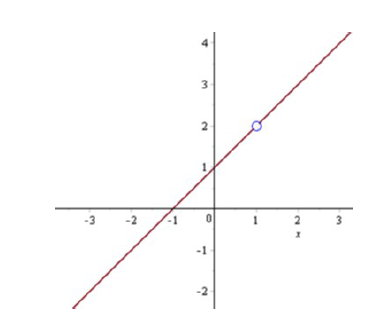
\includegraphics{Figure1}
				\end{image}
			\end{freeResponse}
			
			\item  If $  \lim_{x \to a^-} f(x) = L$, then $  \lim_{x \to a^+} f(x) = L $.
			\begin{freeResponse}
			False.  In the graph below $ \lim_{x \to 2^-} f(x) = -1$ but $ \lim_{x \to 2^+} f(x) = 1$.
			
				\begin{image}
						      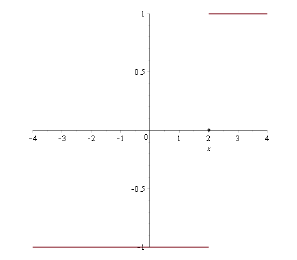
\includegraphics[scale=.7]{Figure2}		
				\end{image}
			\end{freeResponse}
			
			\item  If $ \lim_{x \to a} f(x) = L $ and $  \lim_{x \to a} g(x) = L $, then $f(a) = g(a)$.
			\begin{freeResponse}
			 False.  If we let 
			 
			 	\begin{image}
			       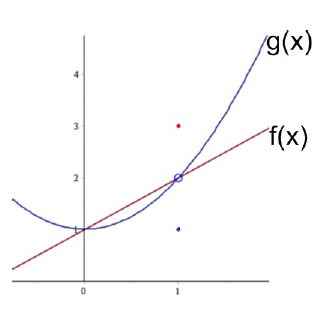
\includegraphics{Figure3}
			 	\end{image}
				
			 we see that $ \lim_{x \to 1} f(x) = \lim_{x \to 1} g(x) = 2$, but $f(1) \ne g(1)$.
			\end{freeResponse}
			
			\item  $ \lim_{x \to a} \frac{f(x)}{g(x)} $ does not exist if $g(a) = 0$.
			\begin{freeResponse}
			False.  If $f(x) = x^3$ and $g(x) = x^2$, then $g(0) = 0$ but 
			$$ \lim_{x \to 0} \frac{f(x)}{g(x)} = \lim_{x \to 0} \frac{x^3}{x^2} = \lim_{x \to 0} x = 0.$$
			\end{freeResponse}
			
			
			
			\end{enumerate}
\end{problem}
	

\end{document} 


















